\documentclass[12pt, a4paper]{report}

%% ─── Packages ────────────────────────────────────────────────────────────────
\usepackage[utf8]{inputenc}
\usepackage[T1]{fontenc}
\usepackage{geometry}
\usepackage{hyperref}
\usepackage{amsmath}
\usepackage{amssymb}
\usepackage{mathtools}
\usepackage{listings}
\usepackage{xcolor}
\usepackage{booktabs}
\usepackage{longtable}
\usepackage{array}
\usepackage{enumitem}
\usepackage{titlesec}
\usepackage{fancyhdr}
\usepackage{graphicx}
\usepackage{float}
\usepackage{tcolorbox}
\usepackage{mdframed}
\usepackage{tikz}
\usetikzlibrary{shapes.geometric, arrows, positioning, calc, fit, backgrounds}

\geometry{
  left=3.2cm, right=3.2cm,
  top=3cm, bottom=3cm,
  headheight=15pt
}

\hypersetup{
  colorlinks=true,
  linkcolor=blue!70!black,
  urlcolor=blue!70!black,
  citecolor=blue!70!black,
  pdftitle={FlowCore: Architecture Blueprint},
  pdfauthor={FlowCore Platform},
}

%% ─── Colors ──────────────────────────────────────────────────────────────────
\definecolor{codebackground}{RGB}{248, 248, 248}
\definecolor{primaryblue}{RGB}{30, 80, 160}
\definecolor{warningred}{RGB}{180, 30, 30}
\definecolor{safegreen}{RGB}{20, 120, 60}
\definecolor{neutralgray}{RGB}{90, 90, 100}

%% ─── Code Listings ───────────────────────────────────────────────────────────
\lstset{
  backgroundcolor=\color{codebackground},
  basicstyle=\ttfamily\small,
  breaklines=true,
  captionpos=b,
  frame=single,
  rulecolor=\color{gray!40},
  numbers=left,
  numberstyle=\tiny\color{gray},
  showstringspaces=false,
  keywordstyle=\color{primaryblue}\bfseries,
  commentstyle=\color{neutralgray}\itshape,
  stringstyle=\color{safegreen},
}

%% ─── Invariant Box ───────────────────────────────────────────────────────────
\newenvironment{invariantbox}[1]{%
  \begin{tcolorbox}[
    colback=red!4!white,
    colframe=warningred,
    title={\textbf{INVARIANT: #1}},
    fonttitle=\small\bfseries
  ]
}{%
  \end{tcolorbox}
}

\newenvironment{principlebox}[1]{%
  \begin{tcolorbox}[
    colback=blue!4!white,
    colframe=primaryblue,
    title={\textbf{PRINCIPLE: #1}},
    fonttitle=\small\bfseries
  ]
}{%
  \end{tcolorbox}
}

\newenvironment{warningbox}{%
  \begin{tcolorbox}[
    colback=yellow!10!white,
    colframe=orange!80!black,
    title={\textbf{ARCHITECTURAL WARNING}},
    fonttitle=\small\bfseries
  ]
}{%
  \end{tcolorbox}
}

%% ─── Header / Footer ─────────────────────────────────────────────────────────
\pagestyle{fancy}
\fancyhf{}
\fancyhead[L]{\small\textit{FlowCore Platform Architecture Blueprint}}
\fancyhead[R]{\small\textit{v1.0.0 — Student Reference Edition}}
\fancyfoot[C]{\thepage}

%% ─── Title ───────────────────────────────────────────────────────────────────
\title{
  \vspace{-1cm}
  {\Large \textsc{FlowCore Platform}} \\[0.4em]
  {\huge \textbf{Architecture Blueprint}} \\[0.6em]
  {\large Deterministic Graph-Based Conversational Workflow Engine} \\[0.4em]
  {\normalsize for WhatsApp-Native Business Automation} \\[1.5em]
  \rule{12cm}{0.4pt} \\[0.6em]
  {\small Version 1.0.0 \quad | \quad Prototype Phase \quad | \quad Architecture-First Document} \\[0.4em]
  {\small \textit{This document constitutes the formal architectural foundation for all implementation phases.}}
}
\author{
  \textsc{FlowCore Engineering} \\
  \small Platform Design \& Systems Architecture
}
\date{\today}

%% ─────────────────────────────────────────────────────────────────────────────
\begin{document}

\maketitle
\thispagestyle{empty}
\newpage

%% ─── Abstract ────────────────────────────────────────────────────────────────
\begin{abstract}
\noindent
\textbf{FlowCore} is a \textit{deterministic, graph-based conversational workflow execution platform} designed to allow small and medium businesses to deploy structured, reliable, and scalable conversational automations over WhatsApp --- without writing code.

The platform is architecturally distinct from both traditional chatbots and autonomous AI agent systems. It does not use AI to control runtime execution. Instead, it constrains AI to a single, isolated role: \textit{workflow graph generation during business onboarding}. Once generated, workflows are validated, simulated, approved, and executed by a fully deterministic runtime engine that owns all state, all FSM transitions, and all execution guarantees.

The design philosophy is: \textbf{``deterministic modular graph execution platform with constrained AI-assisted workflow composition.''} Not an AI chaos system. Not a chatbot. A formally-designed execution kernel.

This document constitutes the full formal architecture foundation. It must be consulted before any implementation phase begins, and preserved across all future implementation conversations to prevent architectural drift.
\end{abstract}

\newpage
\tableofcontents
\newpage

%% ═════════════════════════════════════════════════════════════════════════════
\chapter{Platform Vision and Motivation}
%% ═════════════════════════════════════════════════════════════════════════════

\section{The Problem Space}

Small and medium businesses in emerging markets have a fundamental gap: they need structured, reliable customer interaction workflows --- but they lack the technical capacity to build them. WhatsApp is the dominant communication channel in these markets, yet existing WhatsApp automation solutions fall into two unsatisfactory categories:

\begin{enumerate}
  \item \textbf{Simple keyword-based chatbots}: brittle, stateless, unable to handle real business flows like ordering, payment, and confirmation.
  \item \textbf{AI-orchestrated conversational agents}: unpredictable, unauditable, unable to guarantee execution contracts, and unsafe for business-critical flows like payments.
\end{enumerate}

FlowCore occupies a third, structurally superior position: a \textit{deterministic workflow execution engine} that accepts \textit{business-defined workflow graphs} and executes them with the reliability of traditional software --- while using AI only in a constrained, pre-activation synthesis role.

\section{Platform Goal}

Allow businesses to create \textbf{no-code conversational business workflows} delivered over WhatsApp, with:

\begin{itemize}
  \item deterministic, auditable execution guarantees
  \item structured FSM-based state management
  \item modular, contract-driven workflow composition
  \item domain extensibility (restaurants $\to$ salons $\to$ clinics $\to$ hotels $\to$ logistics)
  \item AI-assisted --- but AI-bounded --- workflow creation
\end{itemize}

\section{Why WhatsApp}

WhatsApp is not a feature choice. It is a structural constraint that shapes the entire execution model:

\begin{itemize}
  \item Interactions are \textit{asynchronous} and \textit{session-scoped}
  \item State must \textit{persist} between turns
  \item Execution must be \textit{recoverable} from mid-session failure
  \item Side effects (payments, order creation) must be \textit{idempotent}
  \item Conversations can be \textit{interrupted} and must resume correctly
\end{itemize}

These constraints make a deterministic, FSM-driven, carry-unit-based architecture not just preferable but \textit{necessary}.

%% ═════════════════════════════════════════════════════════════════════════════
\chapter{System Philosophy}
%% ═════════════════════════════════════════════════════════════════════════════

\section{The Core Philosophical Position}

\begin{principlebox}{The Platform Is a Deterministic Execution Kernel}
FlowCore is not an AI product. It is a \textbf{deterministic execution platform} that uses AI in a single, contained, pre-runtime role. The runtime kernel has zero AI involvement. This is a deliberate, permanent architectural decision.
\end{principlebox}

\section{What This System Is}

\begin{itemize}
  \item A \textbf{graph-based workflow execution engine}: workflows are directed graphs of execution modules, traversed deterministically
  \item A \textbf{contract-driven modular platform}: modules declare what they need and produce; composition is automatic and validated
  \item A \textbf{FSM-enforced stateful runtime}: all session state is managed by a single authoritative FSM engine
  \item A \textbf{carry-unit-propagating execution context}: shared typed state flows through module execution, accumulating outputs
  \item A \textbf{validation-first workflow lifecycle}: no workflow activates without passing structural, dependency, FSM, and simulation validation
\end{itemize}

\section{What This System Is Not}

\begin{warningbox}
\begin{itemize}
  \item \textbf{Not} an autonomous AI agent
  \item \textbf{Not} a freeform LLM orchestration system
  \item \textbf{Not} a traditional keyword-response chatbot
  \item \textbf{Not} a self-modifying runtime system
  \item \textbf{Not} a no-code drag-and-drop UI (initially)
  \item \textbf{Not} a cloud-dependent SaaS platform (initial phase)
\end{itemize}
\end{warningbox}

\section{The Separation of Concerns Doctrine}

The most important philosophical commitment in this platform is the \textbf{absolute separation} between:

\begin{center}
\begin{tabular}{lll}
\toprule
\textbf{Concern} & \textbf{Owned By} & \textbf{Guarantee} \\
\midrule
Runtime execution & Main Execution Backend & Deterministic \\
Session FSM state & FSM Engine (in backend) & Authoritative \\
Carry unit state & Execution Backend & Typed, validated \\
Workflow generation & Generation Backend & AI-bounded \\
WhatsApp transport & Runtime N8N & Thin, dispatch-only \\
Onboarding orchestration & Generation N8N & Lifecycle management \\
\bottomrule
\end{tabular}
\end{center}

No concern may cross its boundary. This is not a preference --- it is an invariant.

%% ═════════════════════════════════════════════════════════════════════════════
\chapter{Core Architectural Principles}
%% ═════════════════════════════════════════════════════════════════════════════

\section{Principle 1: Deterministic Execution}

\begin{principlebox}{Determinism}
Given the same workflow graph, the same session state, and the same carry unit, the execution engine MUST produce the same result every time. No randomness. No AI inference. No runtime mutation of execution logic.
\end{principlebox}

Determinism enables: auditability, replay-safe retries, predictable customer experience, testable execution paths, and trustworthy payment flows.

\section{Principle 2: FSM Authority Centralization}

\begin{invariantbox}{FSM Authority}
Only the Main Execution Backend FSM Engine may mutate conversation FSM state. N8N workflows, AI-generated modules, and external integrations MUST NOT directly mutate FSM state. All state transitions must pass through the FSM Engine's validation layer.
\end{invariantbox}

Without this: state can become inconsistent, multiple systems develop competing FSM assumptions, and execution correctness degrades.

\section{Principle 3: Carry Unit as Execution Contract}

The carry unit is the shared typed execution context that flows through module execution. It is the \textit{memory bus} of the runtime engine.

\begin{align}
\text{Module can execute} &\iff \text{module.requires} \subseteq \text{carry\_unit} \\
\text{After execution:} \quad & \text{carry\_unit}' = \text{carry\_unit} \cup \text{module.produces}
\end{align}

This creates a \textit{lock/key dependency graph}: modules compose automatically when their contracts are compatible, and fail explicitly when dependencies are missing.

\section{Principle 4: Validation Before Activation}

\begin{invariantbox}{No Unvalidated Workflow May Execute}
Every workflow MUST pass the full validation + simulation lifecycle before it may be activated. No exceptions. The lifecycle is: Generate $\to$ Validate $\to$ Simulate $\to$ FSM-Verify $\to$ Dependency-Verify $\to$ Sandbox-Execute $\to$ Approve $\to$ Activate.
\end{invariantbox}

\section{Principle 5: AI as Constrained Proposer}

\begin{principlebox}{AI Role Constraint}
AI (local Llama) is permitted only one role: proposing workflow graphs during onboarding, using valid modules from the module registry. AI output is always treated as an untrusted proposal that must pass full validation before any further lifecycle progression. AI NEVER controls runtime execution.
\end{principlebox}

\section{Principle 6: Module Composability}

Modules are the atomic units of the platform. Each module is:
\begin{itemize}
  \item Self-describing (contract defines inputs, outputs, FSM constraints)
  \item Self-contained (execution handler is isolated)
  \item Composable (contracts enable automatic graph composition)
  \item Side-effect-aware (side effects declared, not hidden)
\end{itemize}

New domains (salons, clinics, hotels) require only new module definitions. No orchestrator rewrites.

\section{Principle 7: Business Isolation}

All data, sessions, workflows, and execution traces are scoped to a \texttt{business\_id}. No business can access another's data, sessions, or workflows. This is enforced at the database query layer, not at the application layer.

\section{Principle 8: Idempotency by Design}

All module executions must declare whether they are idempotent. Non-idempotent modules (e.g., payment initiation) must use idempotency keys to prevent double-execution on retry. The execution engine tracks executed nodes per session.

%% ═════════════════════════════════════════════════════════════════════════════
\chapter{The Four-System Architecture}
%% ═════════════════════════════════════════════════════════════════════════════

\section{Overview}

The platform consists of four completely separated systems, each with its own responsibilities, guarantees, and execution philosophy. These systems communicate only through APIs, contracts, and schemas.

\begin{figure}[H]
\centering
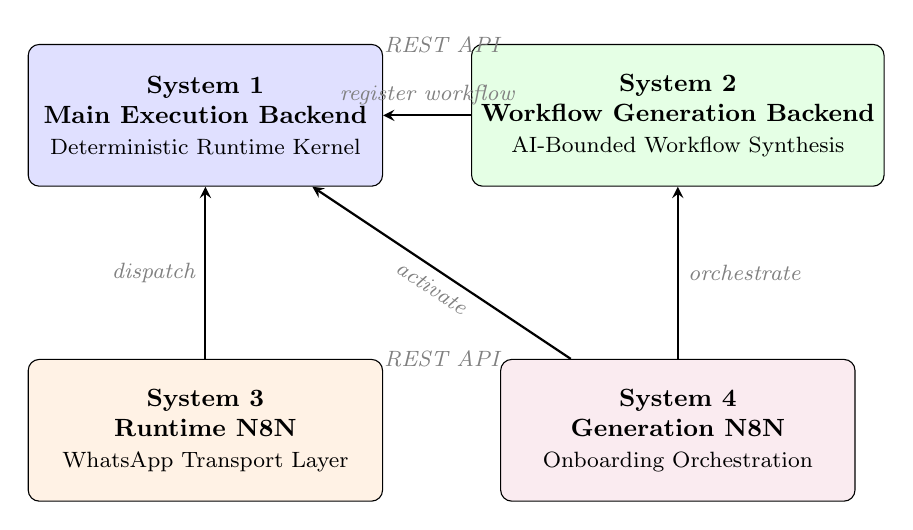
\begin{tikzpicture}[
  box/.style={rectangle, draw, rounded corners=4pt, minimum width=4.5cm, minimum height=1.8cm, align=center, font=\small},
  arrow/.style={->, thick, >=stealth},
  label/.style={font=\footnotesize\itshape, color=gray}
]

%% Boxes
\node[box, fill=blue!12] (exec) at (0, 0) {\textbf{System 1}\\\textbf{Main Execution Backend}\\{\footnotesize Deterministic Runtime Kernel}};
\node[box, fill=green!10] (gen) at (6, 0) {\textbf{System 2}\\\textbf{Workflow Generation Backend}\\{\footnotesize AI-Bounded Workflow Synthesis}};
\node[box, fill=orange!10] (n8n_rt) at (0, -4) {\textbf{System 3}\\\textbf{Runtime N8N}\\{\footnotesize WhatsApp Transport Layer}};
\node[box, fill=purple!8] (n8n_gen) at (6, -4) {\textbf{System 4}\\\textbf{Generation N8N}\\{\footnotesize Onboarding Orchestration}};

%% Arrows
\draw[arrow] (n8n_rt) -- node[label, left]{dispatch} (exec);
\draw[arrow] (gen) -- node[label, above]{register workflow} (exec);
\draw[arrow] (n8n_gen) -- node[label, right]{orchestrate} (gen);
\draw[arrow] (n8n_gen) -- node[label, below, sloped]{activate} (exec);

%% Labels
\node[label] at (3, 0.9) {REST API};
\node[label] at (3, -3.1) {REST API};

\end{tikzpicture}
\caption{Four-System Architecture Overview}
\end{figure}

\section{System 1: Main Execution Backend}

\textbf{Role}: The authoritative, deterministic runtime execution kernel.

\textbf{Technology}: FastAPI, SQLAlchemy, Pydantic, SQLite (dev) / PostgreSQL (prod).

\textbf{Responsibilities}:
\begin{enumerate}
  \item Session management and persistence
  \item FSM authority (sole owner of state transitions)
  \item Graph traversal and execution ordering
  \item Carry unit management
  \item Module registry
  \item Workflow runtime execution (validated workflows only)
  \item Retry and idempotency enforcement
  \item Execution trace and audit logging
  \item Workflow registry and versioning
  \item Business isolation enforcement
\end{enumerate}

\begin{invariantbox}{System 1 Authority}
System 1 is the sole runtime authority. All other systems are subordinate to its contracts. It executes only validated workflows. It owns FSM state exclusively.
\end{invariantbox}

\section{System 2: Workflow Generation Backend}

\textbf{Role}: AI-bounded workflow synthesis engine. Onboarding intelligence layer.

\textbf{Technology}: FastAPI, SQLAlchemy, Pydantic, local Llama via HTTP (localhost:11434).

\textbf{Responsibilities}:
\begin{enumerate}
  \item Business onboarding and configuration collection
  \item Local Llama prompting and response handling
  \item Constrained workflow graph composition (using only valid modules)
  \item Structural validation before submission to System 1
  \item Workflow registration (posting to System 1's registry)
  \item Workflow versioning and lifecycle coordination
\end{enumerate}

\begin{invariantbox}{System 2 Constraint}
System 2 NEVER controls runtime execution. It proposes. System 1 decides. AI output is always an untrusted proposal. Workflows generated here MUST pass System 1 validation before activation.
\end{invariantbox}

\section{System 3: Runtime N8N Orchestration}

\textbf{Role}: Thin WhatsApp transport and dispatch layer for live customer interactions.

\textbf{Responsibilities}:
\begin{enumerate}
  \item WhatsApp webhook ingestion and normalization
  \item Session and business lookup coordination
  \item Execution dispatch to System 1
  \item Transport-level retry handling
  \item Response routing back to customer
\end{enumerate}

\begin{warningbox}
System 3 MUST remain thin. It must never contain business logic, FSM state, or execution authority. Its only role is: receive $\to$ identify $\to$ dispatch $\to$ respond. The moment business logic migrates into N8N, orchestration spaghetti will follow.
\end{warningbox}

\section{System 4: Workflow Generation N8N Orchestration}

\textbf{Role}: Onboarding lifecycle orchestration layer. Manages workflow generation pipeline.

\textbf{Responsibilities}:
\begin{enumerate}
  \item Business onboarding flow orchestration
  \item Workflow generation lifecycle coordination
  \item Validation and simulation orchestration
  \item Approval workflow management
  \item Workflow deployment and activation coordination
\end{enumerate}

\begin{invariantbox}{System 4 Constraint}
System 4 MUST NOT participate in live customer execution. It operates only during onboarding and workflow lifecycle management. It does not own FSM state.
\end{invariantbox}

%% ═════════════════════════════════════════════════════════════════════════════
\chapter{Deterministic Runtime Architecture}
%% ═════════════════════════════════════════════════════════════════════════════

\section{Why Determinism Matters}

The moment runtime execution becomes non-deterministic --- whether through AI inference, conditional branching without guards, or uncontrolled state mutation --- the following guarantees collapse:

\begin{itemize}
  \item Execution cannot be audited
  \item Errors cannot be reproduced
  \item Retries may double-execute side effects
  \item Customer experience becomes unpredictable
  \item Payment and order safety degrades
  \item Debugging becomes impossible at scale
\end{itemize}

Determinism is not a quality-of-life feature. It is a \textit{correctness requirement}.

\section{How Determinism Is Achieved}

\begin{enumerate}
  \item \textbf{Workflow graphs are static}: once activated, a workflow graph does not mutate
  \item \textbf{Module contracts are fixed}: requires/produces do not change at runtime
  \item \textbf{Carry unit evolution is monotonic}: fields are added, never removed mid-session
  \item \textbf{FSM transitions are enumerated}: all legal transitions are pre-defined in the workflow
  \item \textbf{Execution ordering is O(1) compiled lookup}: topological order and node lookups are pre-compiled, removing dynamic graph searching at runtime
  \item \textbf{Idempotency keys prevent re-execution}: non-idempotent modules track execution state
\end{enumerate}

\section{The Execution Loop}

\begin{lstlisting}[language=Python, caption={Pseudocode: Core Execution Loop}]
def execute_step(session, workflow_graph, user_input):
    # 1. Load session state
    carry_unit = session.carry_unit
    fsm_state = session.fsm_state
    current_node = session.current_node

    # 2. Merge user input into carry unit
    carry_unit = carry_unit.merge(normalize(user_input))

    # 3. Determine next executable nodes
    candidates = graph.get_outgoing_edges(current_node)
    next_node = resolve_next(candidates, carry_unit, fsm_state)

    # 4. Validate module preconditions
    module = registry.get(next_node.module_name)
    assert module.requires <= carry_unit.keys()
    assert fsm_state in module.allowed_fsm_states

    # 5. Execute module (deterministically)
    result = module.execute(carry_unit, config=next_node.config)

    # 6. Update carry unit (ONLY via merge, never replace)
    carry_unit = carry_unit.merge(result.outputs)

    # 7. FSM transition (ONLY via FSM engine)
    if next_node.fsm_transition_to:
        fsm_state = fsm_engine.transition(
            from=fsm_state,
            to=next_node.fsm_transition_to
        )

    # 8. Persist session (atomic)
    session.persist(carry_unit, fsm_state, next_node.id)

    # 9. Write execution log (append-only)
    execution_log.append(...)

    return result
\end{lstlisting}

%% ═════════════════════════════════════════════════════════════════════════════
\chapter{The Carry Unit: Typed Execution Context}
%% ═════════════════════════════════════════════════════════════════════════════

\section{Concept}

The carry unit is the \textit{shared, typed, versioned, accumulated execution context} that flows through an entire session's workflow execution. It is the central data structure around which the entire platform is built.

Formally:

\begin{align}
  C_0 &= \{ \text{customer\_phone}, \text{business\_id}, \text{session\_id} \} \\
  C_{n+1} &= C_n \cup \text{module}_n.\text{produces} \\
  \text{module}_n \text{ may execute} &\iff \text{module}_n.\text{requires} \subseteq C_n
\end{align}

\section{Carry Unit Invariants}

\begin{invariantbox}{Carry Unit Invariants}
\begin{enumerate}
  \item The carry unit is \textbf{append-only} within a session. Fields are never removed.
  \item The carry unit is \textbf{typed}. All fields have declared types via module contracts and are verified using a Pydantic schema model.
  \item The carry unit is \textbf{versioned}. Each module execution increments the version.
  \item The carry unit is \textbf{namespaced} per session. Cross-session pollution is impossible.
  \item The carry unit is \textbf{persisted} atomically with each session state update.
  \item The carry unit must \textbf{never be a raw untyped dict} at the contract boundary.
\end{enumerate}
\end{invariantbox}

\section{Initial Carry Unit Fields}

Every session begins with a seeded carry unit containing:

\begin{lstlisting}[language=json, caption={Initial Carry Unit}]
{
  "customer_phone": "+91XXXXXXXXXX",
  "business_id": "01HXYZ...",
  "session_id": "01HXYZ...",
  "workflow_version_id": "01HXYZ...",
  "session_started_at": "2024-01-01T00:00:00Z"
}
\end{lstlisting}

These fields are guaranteed to be present at the start of every session. Modules may depend on them unconditionally.

\section{Carry Unit as Lock/Key Graph}

The carry unit enables a powerful architectural primitive: \textit{automatic module composition} through contract matching.

\begin{figure}[H]
\centering
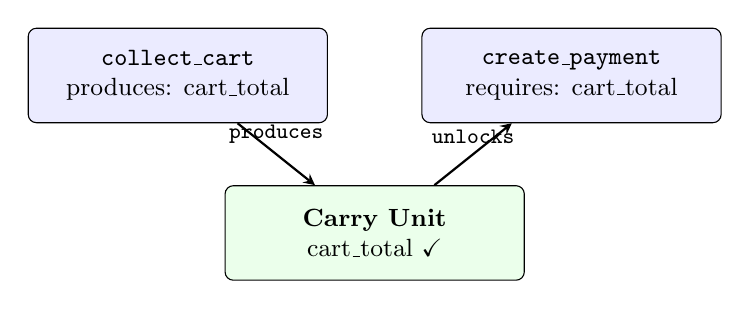
\begin{tikzpicture}[
  module/.style={rectangle, draw, rounded corners=3pt, minimum width=3.8cm, minimum height=1.2cm, align=center, font=\small},
  arrow/.style={->, thick, >=stealth},
  field/.style={font=\footnotesize\ttfamily}
]

\node[module, fill=blue!8] (a) at (0,0) {\texttt{collect\_cart}\\\small produces: cart\_total};
\node[module, fill=blue!8] (b) at (5,0) {\texttt{create\_payment}\\\small requires: cart\_total};
\node[module, fill=green!8] (cu) at (2.5,-2) {\textbf{Carry Unit}\\\small cart\_total $\checkmark$};

\draw[arrow] (a) -- node[above, field]{produces} (cu);
\draw[arrow] (cu) -- node[above, field]{unlocks} (b);

\end{tikzpicture}
\caption{Carry Unit as Lock/Key Composition Mechanism}
\end{figure}

%% ═════════════════════════════════════════════════════════════════════════════
\chapter{Module Contract System}
%% ═════════════════════════════════════════════════════════════════════════════

\section{Module Definition}

Every module in the platform must declare a complete, machine-readable contract:

\begin{lstlisting}[language=json, caption={Full Module Contract}]
{
  "module_name": "create_payment",
  "display_name": "Initiate Payment",
  "version": "1.0.0",
  "domain": "*",
  "requires": [
    "cart_total",
    "customer_phone",
    "order_id"
  ],
  "produces": [
    "payment_url",
    "transaction_id",
    "payment_status"
  ],
  "allowed_fsm_states": ["CHECKOUT"],
  "side_effects": ["payment_initiated", "external_payment_api_called"],
  "is_idempotent": false,
  "expects_user_input": false,
  "retry_config": {
    "max_retries": 3,
    "backoff_strategy": "exponential",
    "idempotency_key_fields": ["order_id", "customer_phone"]
  }
}
\end{lstlisting}

\section{Module Categories}

\begin{longtable}{lll}
\toprule
\textbf{Module} & \textbf{Domain} & \textbf{Purpose} \\
\midrule
\texttt{show\_menu} & restaurant & Display business menu \\
\texttt{collect\_cart} & restaurant & Build customer cart \\
\texttt{calculate\_total} & restaurant & Compute cart total \\
\texttt{create\_order} & restaurant & Persist order \\
\texttt{create\_payment} & * & Initiate payment \\
\texttt{verify\_payment} & * & Confirm payment status \\
\texttt{send\_confirmation} & * & Send order/booking confirmation \\
\texttt{collect\_delivery\_address} & restaurant & Gather delivery info \\
\texttt{check\_availability} & salon/clinic & Check appointment slots \\
\texttt{book\_appointment} & salon/clinic & Reserve appointment \\
\texttt{handle\_faq} & * & Answer FAQ queries \\
\texttt{collect\_feedback} & * & Post-interaction feedback \\
\bottomrule
\end{longtable}

\section{Module Registry}

The module registry is the authoritative catalog of all valid modules. It is:
\begin{itemize}
  \item Loaded at backend startup from code definitions
  \item Persisted to the database for queryability
  \item Read-only at runtime (no runtime module registration)
  \item The \textit{only} source of valid module names for workflow generation
\end{itemize}

\begin{invariantbox}{Module Registry}
The AI workflow generator MUST fetch the current module registry before composing any workflow graph. It may ONLY use module names that exist in the registry. Hallucinated module names must be rejected at validation.
\end{invariantbox}

%% ═════════════════════════════════════════════════════════════════════════════
\chapter{FSM Engine: State Authority}
%% ═════════════════════════════════════════════════════════════════════════════

\section{FSM States (Default: Restaurant Domain)}

\begin{center}
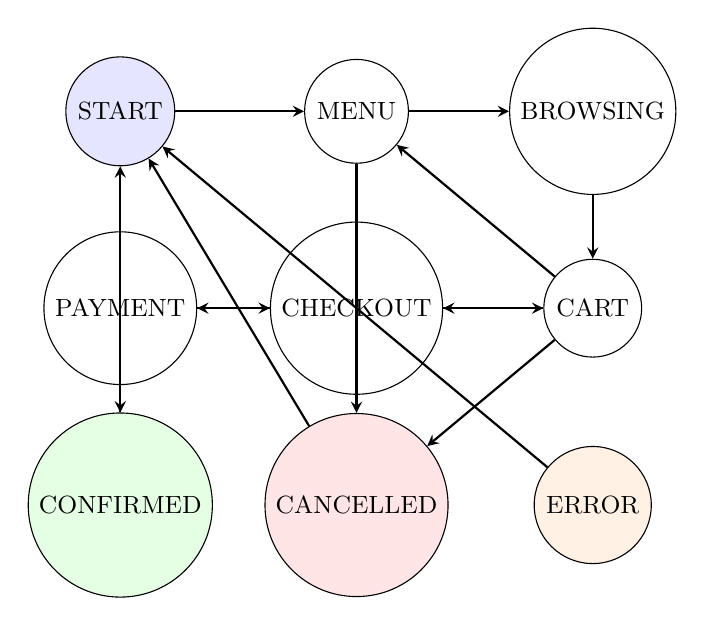
\begin{tikzpicture}[
  state/.style={circle, draw, minimum size=1.2cm, font=\small},
  arrow/.style={->, thick, >=stealth}
]
\node[state, fill=blue!10] (start) at (0, 0) {START};
\node[state] (menu) at (3, 0) {MENU};
\node[state] (browsing) at (6, 0) {BROWSING};
\node[state] (cart) at (6, -2.5) {CART};
\node[state] (checkout) at (3, -2.5) {CHECKOUT};
\node[state] (payment) at (0, -2.5) {PAYMENT};
\node[state, fill=green!10] (confirmed) at (0, -5) {CONFIRMED};
\node[state, fill=red!10] (cancelled) at (3, -5) {CANCELLED};
\node[state, fill=orange!10] (error) at (6, -5) {ERROR};

\draw[arrow] (start) -- (menu);
\draw[arrow] (menu) -- (browsing);
\draw[arrow] (browsing) -- (cart);
\draw[arrow] (cart) -- (checkout);
\draw[arrow] (checkout) -- (payment);
\draw[arrow] (payment) -- (confirmed);
\draw[arrow] (cart) -- (menu);
\draw[arrow] (checkout) -- (cart);
\draw[arrow] (payment) -- (checkout);
\draw[arrow] (menu) -- (cancelled);
\draw[arrow] (cart) -- (cancelled);
\draw[arrow] (confirmed) -- (start);
\draw[arrow] (cancelled) -- (start);
\draw[arrow] (error) -- (start);
\end{tikzpicture}
\caption{Default Restaurant Domain FSM}
\end{center}

\section{FSM Engine Rules}

\begin{invariantbox}{FSM Engine Rules}
\begin{enumerate}
  \item Only the FSM Engine class in System 1 may call \texttt{transition()}.
  \item All transition requests are validated against the workflow-defined transition table.
  \item Invalid transitions raise \texttt{InvalidTransitionError} and abort the execution step.
  \item FSM state is persisted atomically with the session update.
  \item FSM state is loaded fresh from the database on every execution step (no in-memory caching).
  \item Terminal states (CONFIRMED, CANCELLED) may not transition further within the session.
\end{enumerate}
\end{invariantbox}

\section{Custom FSM Definitions}

Workflows may define custom FSM transition tables (for non-restaurant domains). These must be:
\begin{itemize}
  \item Declared explicitly in the workflow graph JSON
  \item Validated for completeness before workflow activation
  \item Complete: every reachable state must have defined outgoing transitions or be marked terminal
\end{itemize}

%% ═════════════════════════════════════════════════════════════════════════════
\chapter{Graph Traversal and Cursor Persistence}
%% ═════════════════════════════════════════════════════════════════════════════

\section{The Traversal Cursor Invariant}

The platform enforces a critical architectural distinction between where the traversal cursor is stored and where it was:

\begin{invariantbox}{Traversal Cursor Invariant (INV-11)}
The persisted \texttt{current\_node\_id} must ALWAYS represent the \textbf{next node waiting for execution} (unresolved node) rather than the node that was just executed.
\end{invariantbox}

Without this invariant, the runtime is unable to handle multi-turn conversations cleanly, as it would re-evaluate a previously executed node's outgoing transitions on every dispatch instead of executing the pending node directly.

\section{Distinguishing USER vs. ALWAYS Transitions}

At the end of executing a node, the runtime engine evaluates the node's outgoing edges and determines how to proceed using three distinct policies:

\begin{enumerate}
  \item \textbf{USER Edges (Non-always Edges)}: If the outgoing edges are conditional on user input (e.g. \texttt{any\_input}, \texttt{input_equals}), the engine pauses traversal, keeps the current node ID as the cursor, and waits for the next dispatch turn where the new user input will be evaluated against these transitions.
  \item \textbf{ALWAYS Edges to User-Input Nodes}: If the outgoing edge is an \texttt{always} transition but the target node expects user input (e.g. \texttt{collect\_cart}, \texttt{collect\_address}), the engine transitions the cursor pointer to the target node, but \textbf{STOPS} traversal immediately without executing it, waiting for next turn's input to feed the target node.
  \item \textbf{ALWAYS Edges to System Nodes}: If the outgoing edge is \texttt{always} and the target node is an automatic/system node (e.g. \texttt{calculate\_total}, \texttt{create_order}), the engine auto-traverses to the target node and executes it immediately in the same turn.
\end{enumerate}

\begin{figure}[H]
\centering
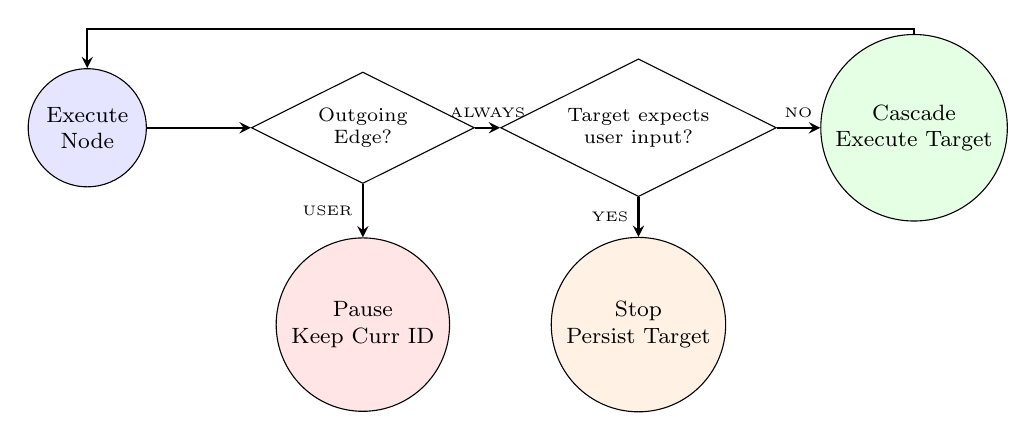
\begin{tikzpicture}[
  node/.style={circle, draw, minimum size=1.5cm, align=center, font=\footnotesize},
  arrow/.style={->, thick, >=stealth},
  decision/.style={diamond, draw, aspect=2, minimum width=2cm, align=center, font=\scriptsize}
]

\node[node, fill=blue!10] (exec) at (0, 0) {Execute\\Node};
\node[decision] (edge) at (3.5, 0) {Outgoing\\Edge?};
\node[node, fill=red!10] (pause) at (3.5, -2.5) {Pause\\Keep Curr ID};
\node[decision] (target) at (7, 0) {Target expects\\user input?};
\node[node, fill=orange!10] (stop) at (7, -2.5) {Stop\\Persist Target};
\node[node, fill=green!10] (cascade) at (10.5, 0) {Cascade\\Execute Target};

\draw[arrow] (exec) -- (edge);
\draw[arrow] (edge) -- node[left, font=\tiny]{USER} (pause);
\draw[arrow] (edge) -- node[above, font=\tiny]{ALWAYS} (target);
\draw[arrow] (target) -- node[left, font=\tiny]{YES} (stop);
\draw[arrow] (target) -- node[above, font=\tiny]{NO} (cascade);
\draw[arrow] (cascade) |- ($(exec.north) + (0, 0.5)$) -| (exec.north);

\end{tikzpicture}
\caption{Traversal Decision Flow Chart}
\end{figure}

%% ═════════════════════════════════════════════════════════════════════════════
\chapter{Workflow Lifecycle}
%% ═════════════════════════════════════════════════════════════════════════════

\section{Full Lifecycle}

\begin{center}
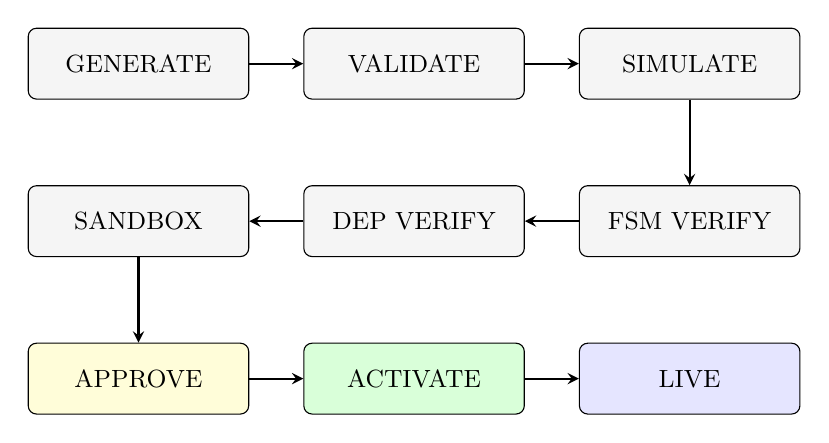
\begin{tikzpicture}[
  stage/.style={rectangle, draw, rounded corners=3pt, minimum width=2.8cm, minimum height=0.9cm, align=center, font=\small, fill=gray!8},
  arrow/.style={->, thick, >=stealth}
]
\node[stage] (gen) at (0,0) {GENERATE};
\node[stage] (val) at (3.5,0) {VALIDATE};
\node[stage] (sim) at (7,0) {SIMULATE};
\node[stage] (fsm) at (7,-2) {FSM VERIFY};
\node[stage] (dep) at (3.5,-2) {DEP VERIFY};
\node[stage] (sand) at (0,-2) {SANDBOX};
\node[stage, fill=yellow!15] (app) at (0,-4) {APPROVE};
\node[stage, fill=green!15] (act) at (3.5,-4) {ACTIVATE};
\node[stage, fill=blue!10] (live) at (7,-4) {LIVE};

\draw[arrow] (gen) -- (val);
\draw[arrow] (val) -- (sim);
\draw[arrow] (sim) -- (fsm);
\draw[arrow] (fsm) -- (dep);
\draw[arrow] (dep) -- (sand);
\draw[arrow] (sand) -- (app);
\draw[arrow] (app) -- (act);
\draw[arrow] (act) -- (live);
\end{tikzpicture}
\caption{Workflow Lifecycle: Generate to Live}
\end{center}

\section{Workflow Status Enum}

\begin{lstlisting}[language=Python]
class WorkflowStatus(str, Enum):
    DRAFT       = "DRAFT"       # Generated, not yet validated
    VALIDATING  = "VALIDATING"  # Structural validation in progress
    SIMULATING  = "SIMULATING"  # Simulation running
    APPROVED    = "APPROVED"    # Passed all checks, awaiting activation
    ACTIVE      = "ACTIVE"      # Live — executing for customers
    DEPRECATED  = "DEPRECATED"  # Superseded by newer version
    FAILED      = "FAILED"      # Validation or simulation failure
\end{lstlisting}

\section{Versioning Strategy}

\begin{itemize}
  \item Each workflow version is \textit{immutable} once activated
  \item Version numbers are monotonically increasing integers per business
  \item At most one version per business may have \texttt{is\_current = True}
  \item Activating a new version atomically deprecates the old one
  \item Execution logs reference \texttt{workflow\_version\_id} permanently
  \item In-progress sessions may complete on their original version
\end{itemize}

%% ═════════════════════════════════════════════════════════════════════════════
\chapter{Workflow Generation: Constrained AI Synthesis}
%% ═════════════════════════════════════════════════════════════════════════════

\section{Why Constrained Generation}

Unconstrained LLM generation of workflow logic is dangerous:
\begin{itemize}
  \item LLMs hallucinate module names, contract fields, and FSM states
  \item Generated logic may bypass security boundaries
  \item Generated code is untestable before execution
  \item Arbitrary code generation creates supply chain risks
  \item Self-modifying runtime logic is fundamentally unsafe
\end{itemize}

Constrained generation solves these by making the LLM a \textit{graph planner}, not a \textit{code generator}:
\begin{itemize}
  \item LLM may only select from registered module names
  \item LLM may only reference valid FSM states
  \item LLM output is a structured JSON graph, not executable code
  \item All LLM output passes through validation before any use
\end{itemize}

\section{Local Llama Integration}

\begin{lstlisting}[language=Python, caption={Local Llama Call Pattern}]
# System 2 only — never in System 1
response = httpx.post(
    "http://localhost:11434/api/generate",
    json={
        "model": "llama3",
        "prompt": build_generation_prompt(
            business_config=business_config,
            available_modules=module_registry.list_all(),
            fsm_states=FSMEngine.all_states(),
            constraints=GENERATION_CONSTRAINTS,
        ),
        "stream": False,
        "format": "json",
    }
)
\end{lstlisting}

\section{Generation Prompt Constraints}

The generation prompt must explicitly communicate to the LLM:
\begin{enumerate}
  \item The exact list of available module names (no others permitted)
  \item The valid FSM states for this business domain
  \item The required output JSON schema (WorkflowGraphSchema)
  \item The constraint that no executable code may be generated
  \item The constraint that all module requires/produces must be honored
\end{enumerate}

%% ═════════════════════════════════════════════════════════════════════════════
\chapter{Database Architecture}
%% ═════════════════════════════════════════════════════════════════════════════

\section{Schema Overview}

\begin{longtable}{lll}
\toprule
\textbf{Table} & \textbf{Purpose} & \textbf{Key Constraint} \\
\midrule
\texttt{businesses} & Business registry & \texttt{whatsapp\_number} unique \\
\texttt{workflow\_versions} & Immutable workflow snapshots & Version + business unique \\
\texttt{module\_registry} & Module catalog & \texttt{name} unique \\
\texttt{sessions} & Active conversations & FSM state owned here \\
\texttt{execution\_logs} & Append-only execution traces & Never mutated \\
\texttt{orders} & Domain: restaurant orders & Scoped to session + business \\
\texttt{payments} & Payment records & \texttt{idempotency\_key} unique \\
\bottomrule
\end{longtable}

\section{Migration Strategy}

\begin{itemize}
  \item Development: SQLite via \texttt{aiosqlite}
  \item Production: PostgreSQL (change \texttt{DATABASE\_URL} only)
  \item No SQLite-specific SQL or types used anywhere
  \item All schema changes via Alembic migrations
  \item ORM models use only SQLAlchemy-portable column types
\end{itemize}

%% ═════════════════════════════════════════════════════════════════════════════
\chapter{Durability: Journaling and Exactly-Once Side Effects}
%% ═════════════════════════════════════════════════════════════════════════════

\section{Write-Ahead Execution Journaling}

To guarantee session durability and recoverability in the event of hardware or database node crashes, System 1 implements a Write-Ahead Journaling (WAL) schema. Every step of execution writes intent markers and stage commitments to the database before modifying downstream registers:

\begin{lstlisting}[language=Python]
class ExecutionJournal(Base):
    __tablename__ = "execution_journals"
    id = Column(String, primary key=True, default=generate_uuid)
    session_id = Column(String, ForeignKey("sessions.id"))
    node_id = Column(String)
    event_type = Column(String)  # BEGIN_NODE, MODULE_EXECUTED, FSM_TRANSITION, SNAPSHOT_WRITTEN, NODE_COMMITTED, NODE_FAILED
    payload_json = Column(Text)
    timestamp = Column(DateTime, default=datetime.utcnow)
\end{lstlisting}

During traversal, these markers record the state boundary of the active node. If a crash occurs mid-execution, a recovery agent parses the journal to replay intents safely or resume from the last successful \texttt{SNAPSHOT\_WRITTEN}.

\section{Exactly-Once Side Effect Semantics}

Side effects generated by non-idempotent modules (like hitting external payment gateways or sending notifications) represent high-risk operations. FlowCore guarantees exactly-once execution through a decentralized event bus and idempotent registry keys:

\begin{lstlisting}[language=Python]
class ExternalOperation(Base):
    __tablename__ = "external_operations"
    idempotency_key = Column(String, primary key=True)
    session_id = Column(String)
    status = Column(String)  # INTENT, COMPLETED, FAILED
    response_json = Column(Text)
    completed_at = Column(DateTime)
\end{lstlisting}

Before dispatching an external payload, the system registers the intent using a deterministic idempotency key. If a concurrent retry is dispatched, the system blocks the request or returns the cached response if already completed.

%% ═════════════════════════════════════════════════════════════════════════════
\chapter{Platform Invariants}
%% ═════════════════════════════════════════════════════════════════════════════

\section{The Permanent Laws}

These invariants must be preserved across every implementation phase, every conversation, and every future evolution of the platform:

\begin{invariantbox}{INV-01: FSM Authority}
Only System 1's FSM Engine may transition session FSM state. No other system, module, or external call may mutate \texttt{session.fsm\_state} directly.
\end{invariantbox}

\begin{invariantbox}{INV-02: Carry Unit Append-Only}
Carry unit fields are never removed within a session. They are only added. The carry unit version increments monotonically.
\end{invariantbox}

\begin{invariantbox}{INV-03: No Unvalidated Workflow Execution}
System 1 MUST reject execution requests for workflows that do not have \texttt{status = ACTIVE}. Draft, failed, and pending workflows may not be executed.
\end{invariantbox}

\begin{invariantbox}{INV-04: AI Never Controls Runtime}
No LLM call may occur within System 1's execution path. AI is confined to System 2, and only during workflow generation, not execution.
\end{invariantbox}

\begin{invariantbox}{INV-05: Module Contract Immutability at Runtime}
Module contracts (requires, produces, allowed\_fsm\_states) may not change after a workflow version is activated. Changes require a new module version and a new workflow version.
\end{invariantbox}

\begin{invariantbox}{INV-06: Business Isolation}
All database queries in System 1 must include \texttt{business\_id} as a filter. Cross-business data access is never permitted.
\end{invariantbox}

\begin{invariantbox}{INV-07: Execution Log Immutability}
Execution log rows are append-only. They are never updated or deleted. They are the permanent audit trail of the platform.
\\
\end{invariantbox}

\begin{invariantbox}{INV-08: Idempotency for Non-Idempotent Modules}
Before executing any module where \texttt{is\_idempotent = false}, the engine must check whether this module has already completed for this session via the execution log.
\end{invariantbox}

\begin{invariantbox}{INV-09: Graph is Acyclic at Activation}
No workflow may be activated if its graph contains a cycle. Cycle detection must pass as part of the validation pipeline.
\end{invariantbox}

\begin{invariantbox}{INV-10: System Separation Must Be Preserved}
Systems 1 and 2 must never share internal code, internal state, or direct function calls. They communicate only through HTTP APIs and shared schema contracts.
\end{invariantbox}

%% ═════════════════════════════════════════════════════════════════════════════
\chapter{Implementation Phase Strategy}
%% ═════════════════════════════════════════════════════════════════════════════

\section{Phase Ordering}

\begin{longtable}{llp{8cm}}
\toprule
\textbf{Phase} & \textbf{Name} & \textbf{Scope} \\
\midrule
1 & Main Execution Backend & Session management, FSM engine, carry unit, module registry, graph traversal, execution tracing, workflow registry, business isolation, retry/idempotency \\
\midrule
2 & Validation + Simulation & Graph cycle detection, dependency validation, FSM verification, simulation engine, sandbox execution, activation lifecycle \\
\midrule
3 & Workflow Generation Backend & Business onboarding, local Llama integration, constrained graph composition, module-aware prompting, workflow registration \\
\midrule
4 & N8N Orchestration Workflows & Runtime N8N (System 3), Generation N8N (System 4), webhook ingestion, dispatch flows, onboarding orchestration \\
\midrule
5 & Dashboard + Analytics & Owner dashboard, execution analytics, workflow performance, conversation monitoring \\
\bottomrule
\end{longtable}

\section{Phase 1 Must Stabilize Before Phase 2}

Phase 1 is the foundation. Phases 2–5 depend on it. The following must be stable before Phase 2 begins:
\begin{itemize}
  \item Module contract schema (Pydantic)
  \item Carry unit schema and merge semantics
  \item FSM engine interface and transition table format
  \item Workflow graph schema (nodes, edges, entry point)
  \item Session data model
  \item Execution log schema
  \item All invariants enforced in code
\end{itemize}

\section{Continuity Contract}

Future implementation conversations must begin by reading:
\begin{enumerate}
  \item This document (\texttt{MASTER\_ARCHITECTURE.tex})
  \item \texttt{PLATFORM\_INVARIANTS.md}
  \item The most recent \texttt{PHASE\_COMPLETION\_REPORT.md}
  \item \texttt{ARCHITECTURE\_SPEC.md}
\end{enumerate}

This is the \textit{continuity protocol}. Without it, architectural drift will occur.

%% ═════════════════════════════════════════════════════════════════════════════
\chapter{Scalability and Future Vision}
%% ═════════════════════════════════════════════════════════════════════════════

\section{Database Migration Path}

\begin{itemize}
  \item Phase 1--3: SQLite + aiosqlite (local dev)
  \item Phase 4+: PostgreSQL (production readiness)
  \item No code changes required — only \texttt{DATABASE\_URL}
  \item Alembic migrations handle schema evolution
\end{itemize}

\section{Domain Expansion}

The module-contract architecture enables domain expansion to salons, clinics, and hotels by defining new modules without modifying the execution core engine.

\section{Guide for Students: Step-by-Step Build Instructions}

For a student attempting to replicate this architecture, proceed in this exact sequence:

\begin{enumerate}
  \item \textbf{Setup Dependencies}: Initialize a virtual environment and install FastAPI, Uvicorn, SQLAlchemy (with aiosqlite), and Pydantic. Set up a testing database in-memory with Pytest.
  \item \textbf{Implement the Context Bus}: Create the Pydantic schemas for the Carry Unit, establishing deep-nested typing for namespaces (like \texttt{order}, \texttt{customer}, \texttt{payment}). Write the merge patch utility.
  \item \textbf{Implement Module Registry}: Write the base module class, inputs/outputs verification routines, and load implementations (such as a simple menu viewer and a mock payment provider).
  \item \textbf{Construct the Traverser}: Write the core recursion/iteration loop in traversal. Ensure you verify \texttt{expects_user_input} to handle cursor stops cleanly.
  \item \textbf{Verify with Tests}: Write tests validating edge cascade rules, transactional rollbacks via database savepoints, and metric captures.
\end{enumerate}

\end{document}
